    \documentclass[dvipsnames]{beamer}
    \usetheme{Madrid}
    \usefonttheme{professionalfonts}
    \usepackage{
        amsmath,
        amssymb,
        fouriernc, % fourier font w/ new century book
        fancyhdr, % page styling
        lastpage, % footer fanciness
        hyperref, % various links
        setspace, % line spacing
        amsthm, % newtheorem and proof environment
        mathtools, % \Aboxed for boxing inside aligns, among others
        float, % Allow [H] figure env alignment
        enumerate, % Allow custom enumerate numbering
        graphicx, % allow includegraphics with more filetypes
        wasysym, % \smiley!
        upgreek, % \upmu for \mum macro
        listings, % writing TrueType fonts and including code prettily
        tikz, % drawing things
        booktabs, % \bottomrule instead of hline apparently
        cancel % can cancel things out!
    }
    \usepackage[
        labelfont=bf, % caption names are labeled in bold
        font=scriptsize % smaller font for captions
    ]{caption}
    \usepackage[font=scriptsize]{subcaption} % subfigures

    \newcommand*{\scinot}[2]{#1\times10^{#2}}
    \newcommand*{\dotp}[2]{\left<#1\,\middle|\,#2\right>}
    \newcommand*{\rd}[2]{\frac{\mathrm{d}#1}{\mathrm{d}#2}}
    \newcommand*{\pd}[2]{\frac{\partial#1}{\partial#2}}
    \newcommand*{\rtd}[2]{\frac{\mathrm{d}^2#1}{\mathrm{d}#2^2}}
    \newcommand*{\ptd}[2]{\frac{\partial^2 #1}{\partial#2^2}}
    \newcommand*{\md}[2]{\frac{\mathrm{D}#1}{\mathrm{D}#2}}
    \newcommand*{\pvec}[1]{\vec{#1}^{\,\prime}}
    \newcommand*{\svec}[1]{\vec{#1}\;\!}
    \newcommand*{\bm}[1]{\boldsymbol{\mathbf{#1}}}
    \newcommand*{\ang}[0]{\;\text{\AA}}
    \newcommand*{\mum}[0]{\;\upmu \mathrm{m}}
    \newcommand*{\at}[1]{\left.#1\right|}

    \let\Re\undefined
    \let\Im\undefined
    \DeclareMathOperator{\Res}{Res}
    \DeclareMathOperator{\Re}{Re}
    \DeclareMathOperator{\Im}{Im}
    \DeclareMathOperator{\Log}{Log}
    \DeclareMathOperator{\Arg}{Arg}
    \DeclareMathOperator{\Tr}{Tr}
    \DeclareMathOperator{\E}{E}
    \DeclareMathOperator{\Var}{Var}
    \DeclareMathOperator*{\argmin}{argmin}
    \DeclareMathOperator*{\argmax}{argmax}
    \DeclareMathOperator{\sgn}{sgn}
    \DeclareMathOperator{\diag}{diag\;}

    \DeclarePairedDelimiter\bra{\langle}{\rvert}
    \DeclarePairedDelimiter\ket{\lvert}{\rangle}
    \DeclarePairedDelimiter\abs{\lvert}{\rvert}
    \DeclarePairedDelimiter\ev{\langle}{\rangle}
    \DeclarePairedDelimiter\p{\lparen}{\rparen}
    \DeclarePairedDelimiter\s{\lbrack}{\rbrack}
    \DeclarePairedDelimiter\z{\lbrace}{\rbrace}

    % \everymath{\displaystyle} % biggify limits of inline sums and integrals
    \tikzstyle{circ} % usage: \node[circ, placement] (label) {text};
        = [draw, circle, fill=white, node distance=3cm, minimum height=2em]
    \definecolor{commentgreen}{rgb}{0,0.6,0}
    \lstset{
        basicstyle=\ttfamily\footnotesize,
        frame=single,
        numbers=left,
        showstringspaces=false,
        keywordstyle=\color{blue},
        stringstyle=\color{purple},
        commentstyle=\color{commentgreen},
        morecomment=[l][\color{magenta}]{\#}
    }

\begin{document}

\title[Dissipating Disk]{Outcomes of Generating Planetary Obliquities Through a Dissipating Disk}
\subtitle{Group Meeting, Sep 13, 2019}
\author{Yubo Su}

\maketitle

\begin{frame}
    \frametitle{Background}
    \framesubtitle{Problem Setup}

    \begin{columns}
        \begin{column}{0.5\textwidth}
            \begin{figure}[t]
                \centering
                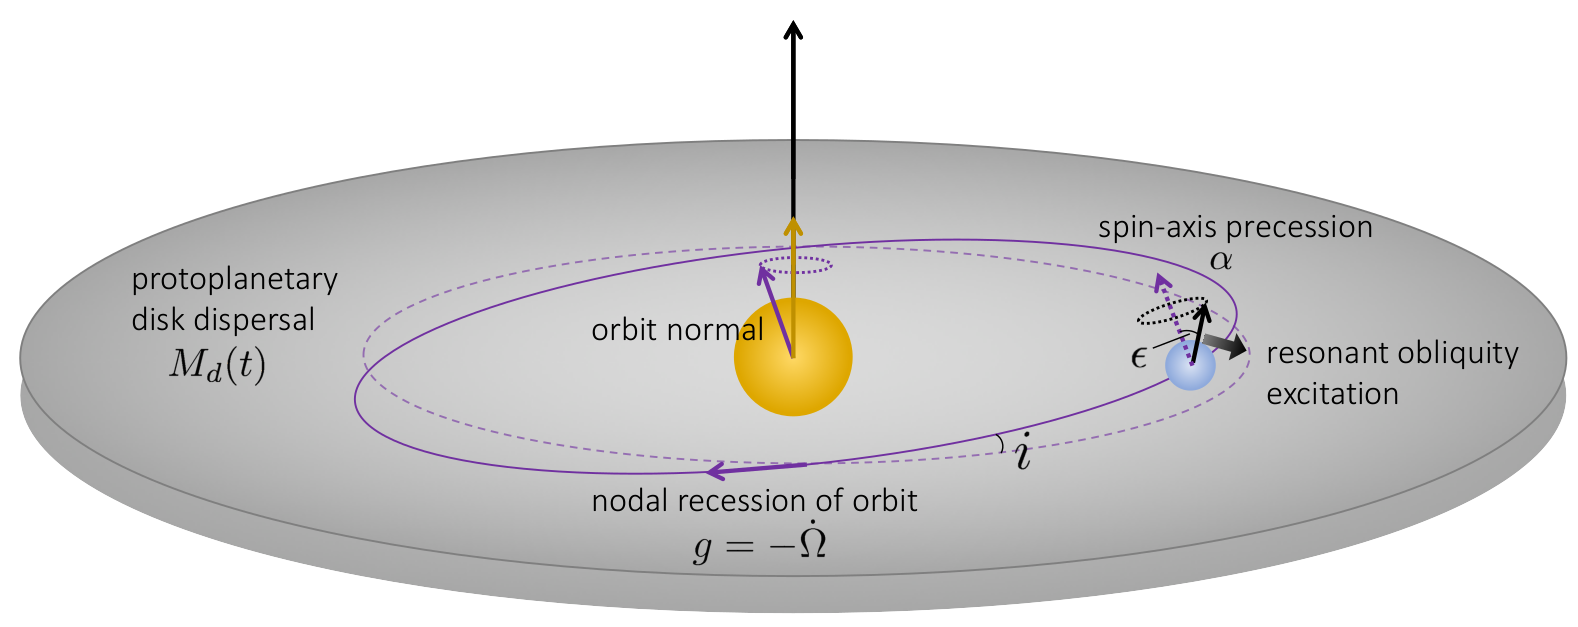
\includegraphics[width=\textwidth]{1millholland_disk.png}
                \caption{Millholland \& Batygin, 2019. Three vectors
                $\hat{s}(t), \hat{l}, \hat{l}_d$.}
            \end{figure}
        \end{column}
        \begin{column}{0.5\textwidth}
            \begin{figure}[t]
                \centering
                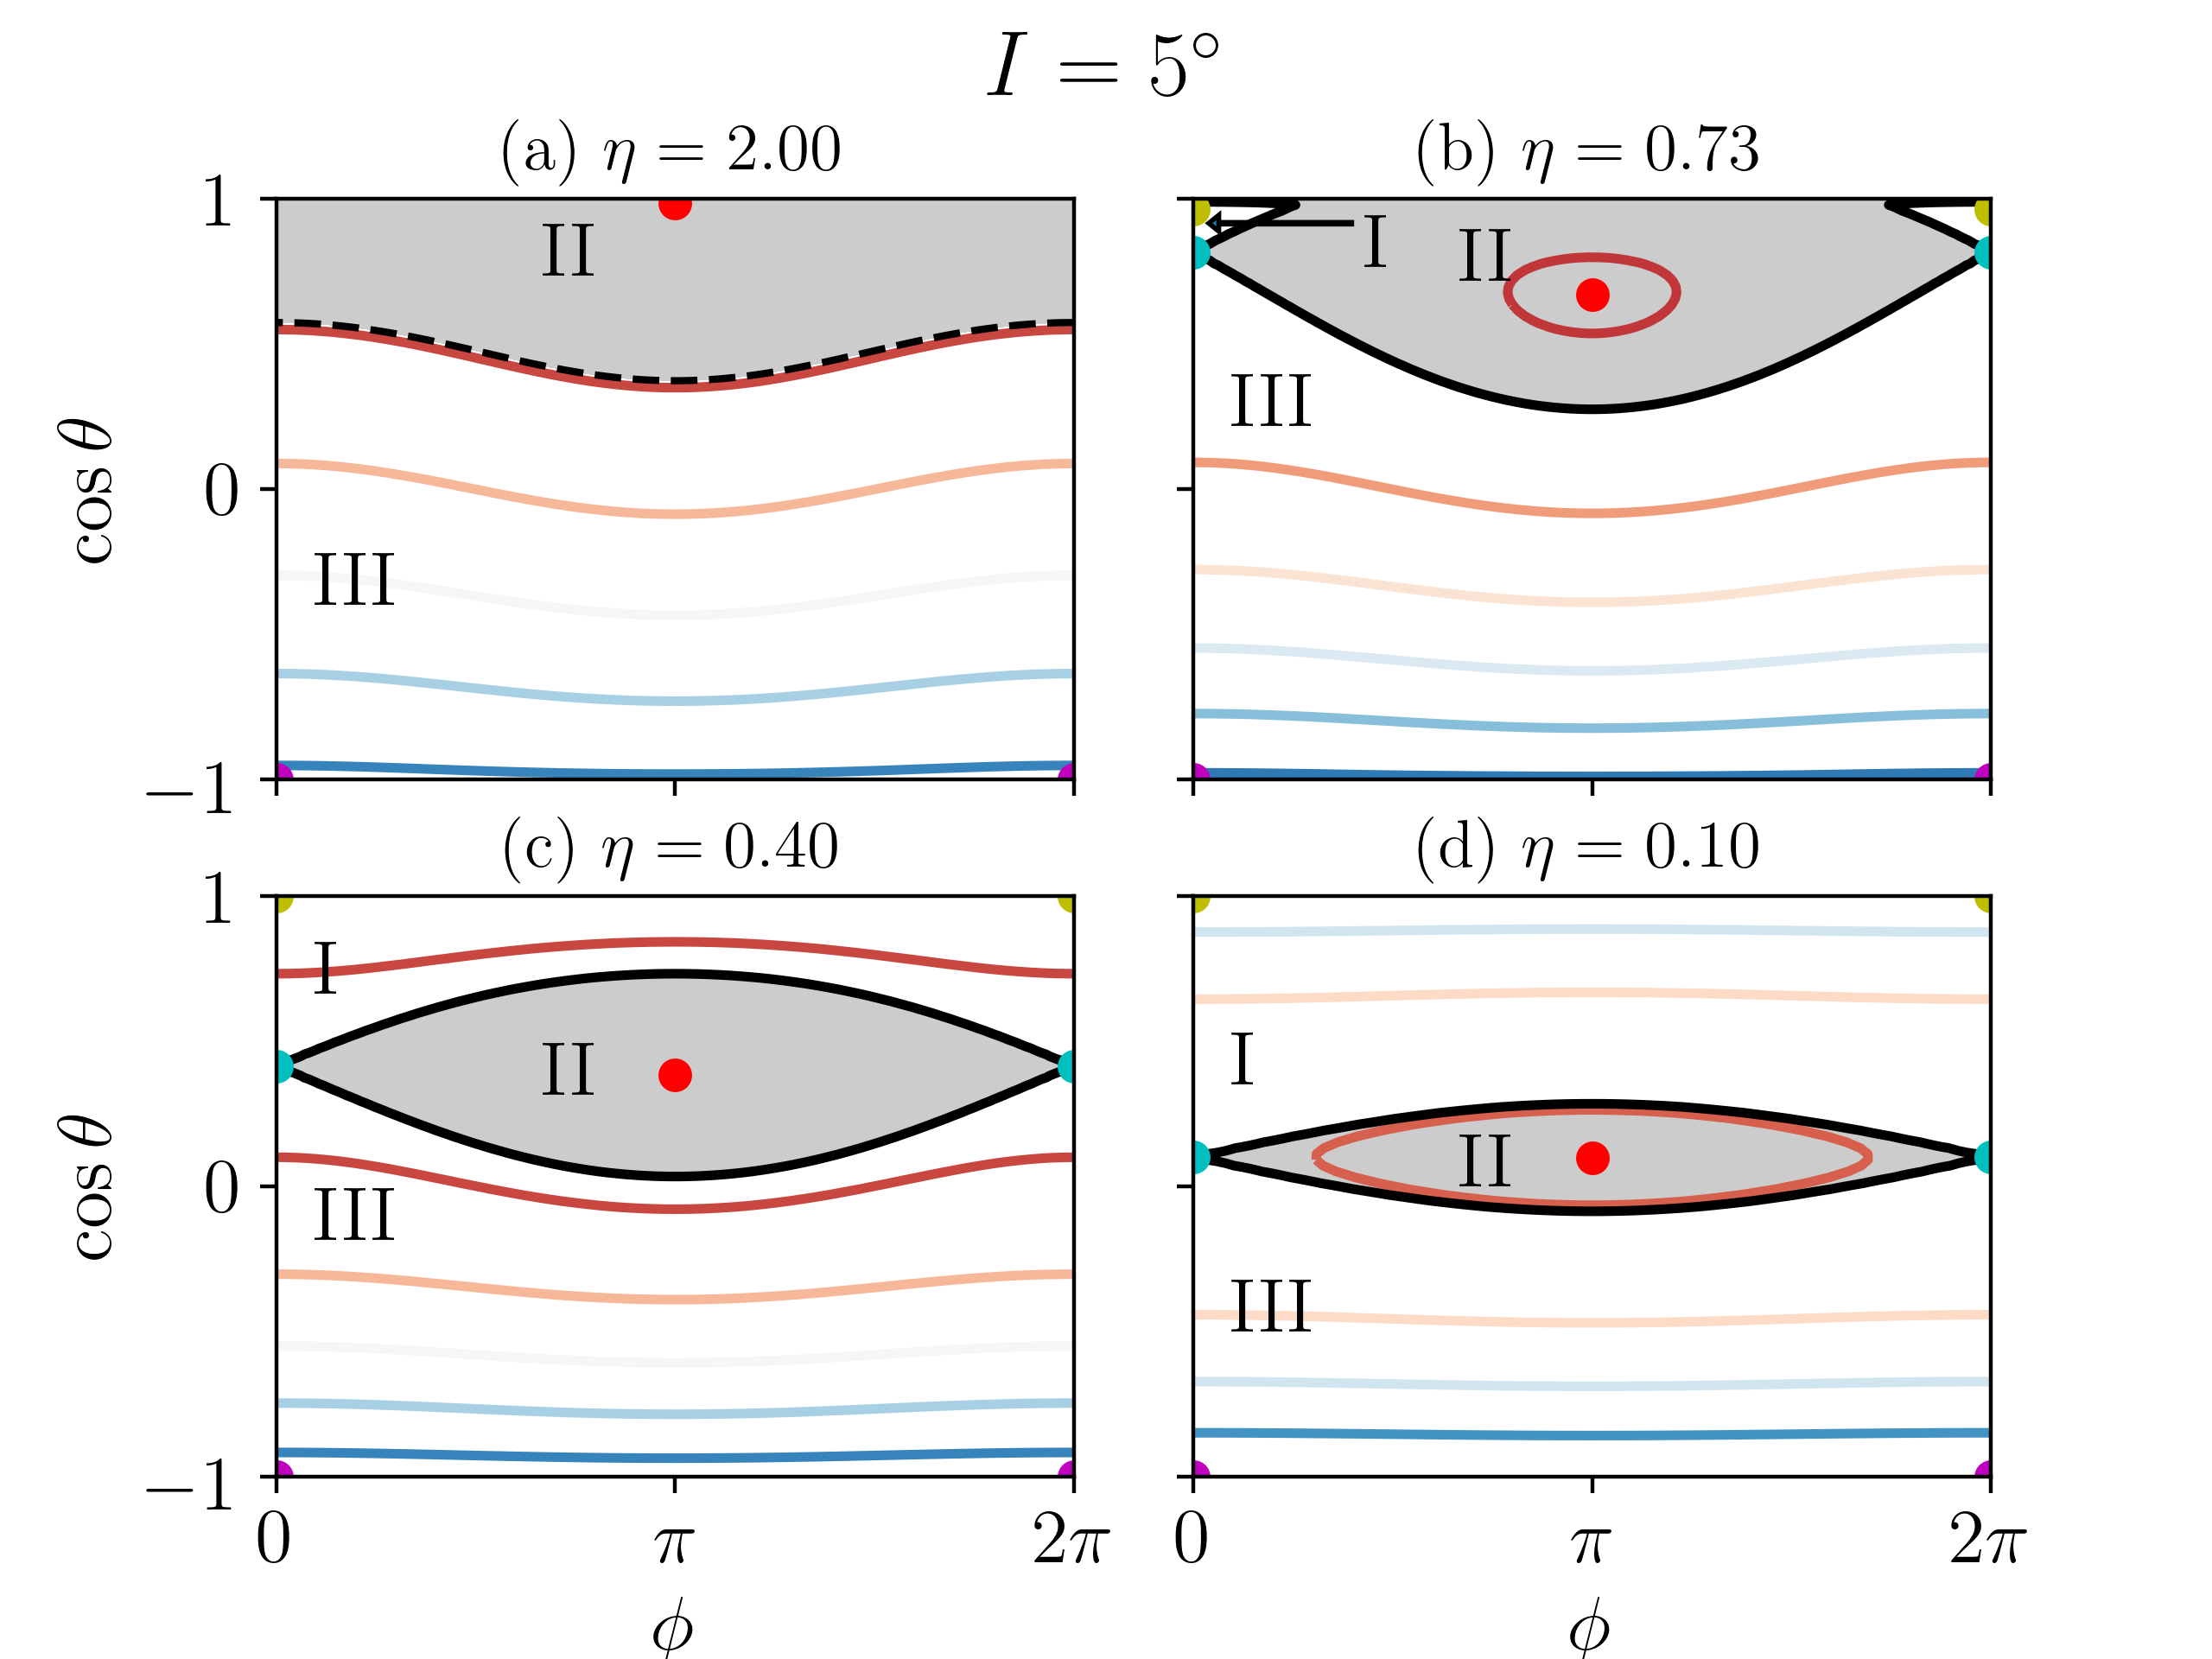
\includegraphics[width=\textwidth]{../../initial/0_eta/1contours_flip.png}
                \caption{$H(\hat{s})$, where $\eta = -\frac{g}{\alpha}$.}
            \end{figure}
        \end{column}
    \end{columns}
\end{frame}

\begin{frame}
    \frametitle{Background}
    \framesubtitle{Existing Work}

    \begin{columns}
        \begin{column}{0.5\textwidth}
            \begin{figure}[t]
                \centering
                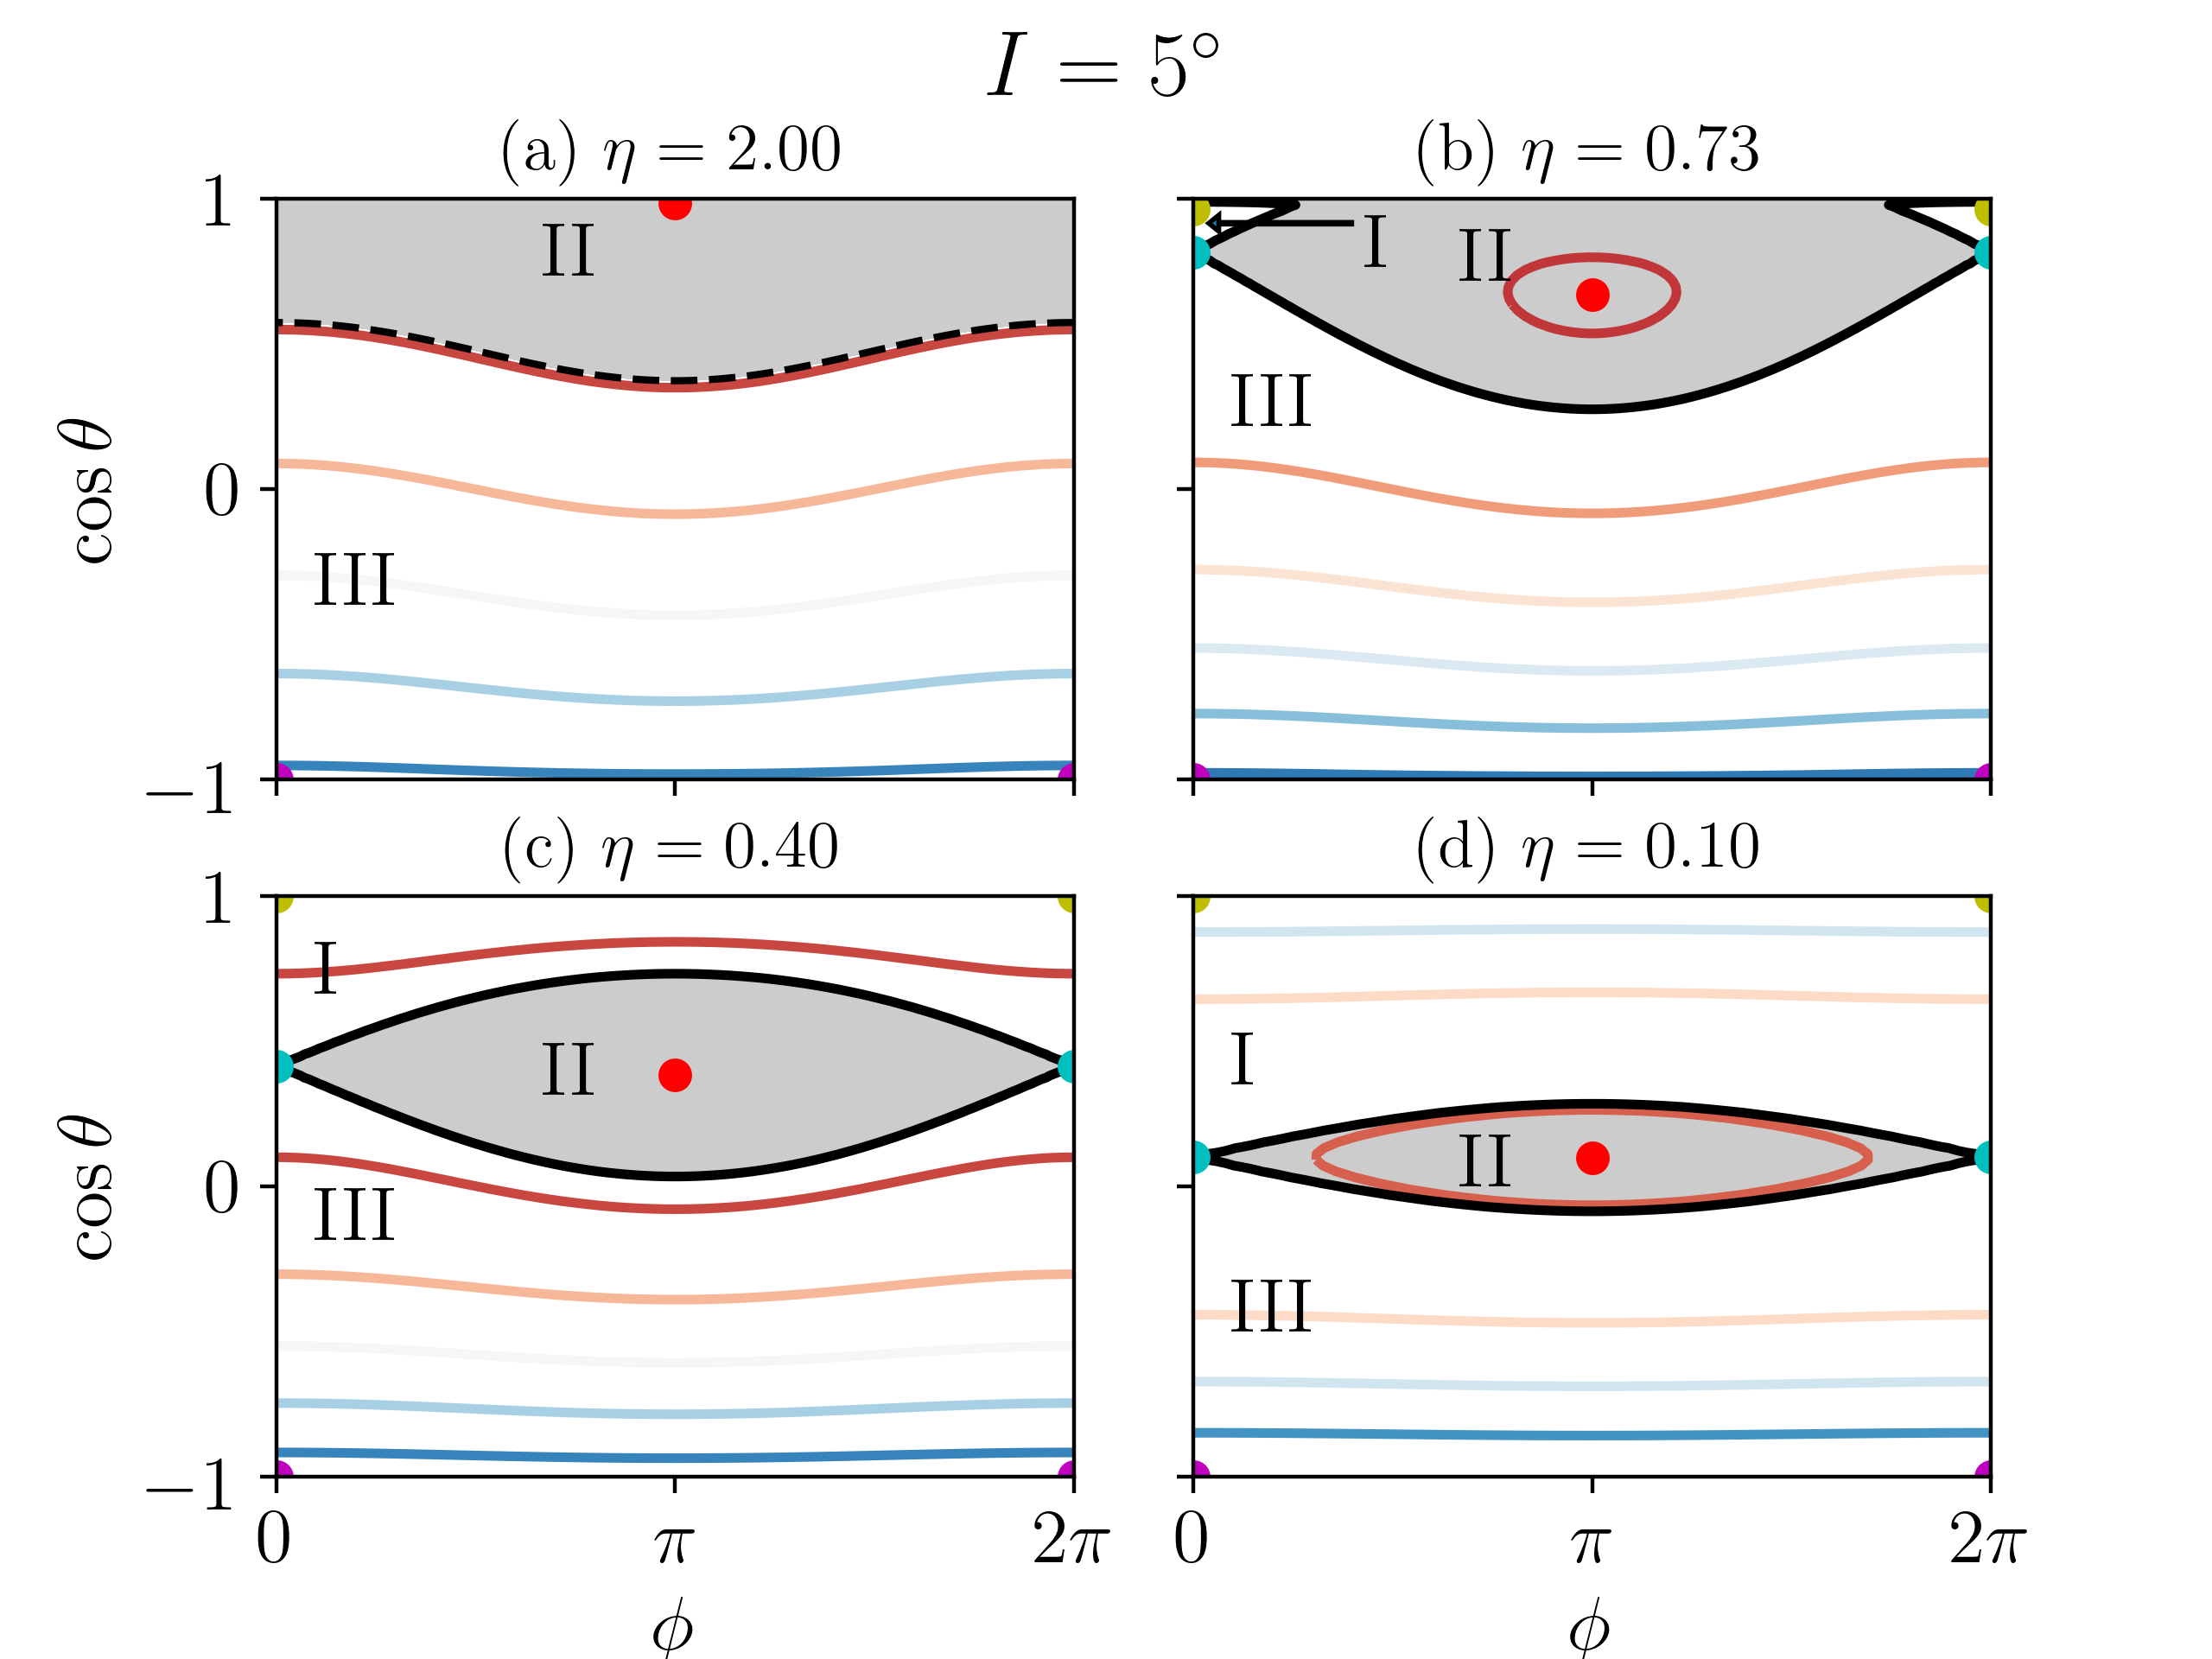
\includegraphics[width=\textwidth]{../../initial/0_eta/1contours_flip.png}
            \end{figure}
            {\scriptsize
            \begin{align*}
                \cos I &= \hat{l} \cdot \hat{l}_d,&
                \theta_{sd, i} &= \hat{s}(t=0) \cdot \hat{l}_d,\\
                \theta_{sl, f} &= \hat{s}(t=t_f) \cdot \hat{l}.
            \end{align*}}
        \end{column}
        \begin{column}{0.5\textwidth}
            \begin{itemize}
                \item Let $\dot{\eta} = -\epsilon\alpha\eta$.

                \item What is $\theta_{sd, f}\p*{\theta_{sd, i}, \epsilon}$?

                \item Millholland \& Batygin 2019: $\epsilon$ dependence,
                    adiabatic vs non-adiabatic regime. No $\theta_{sd, i}$
                    variation.
            \end{itemize}
        \end{column}
    \end{columns}
\end{frame}

\begin{frame}
    \frametitle{Results}
    \framesubtitle{Adiabatic}

    \begin{figure}[t]
        \centering
        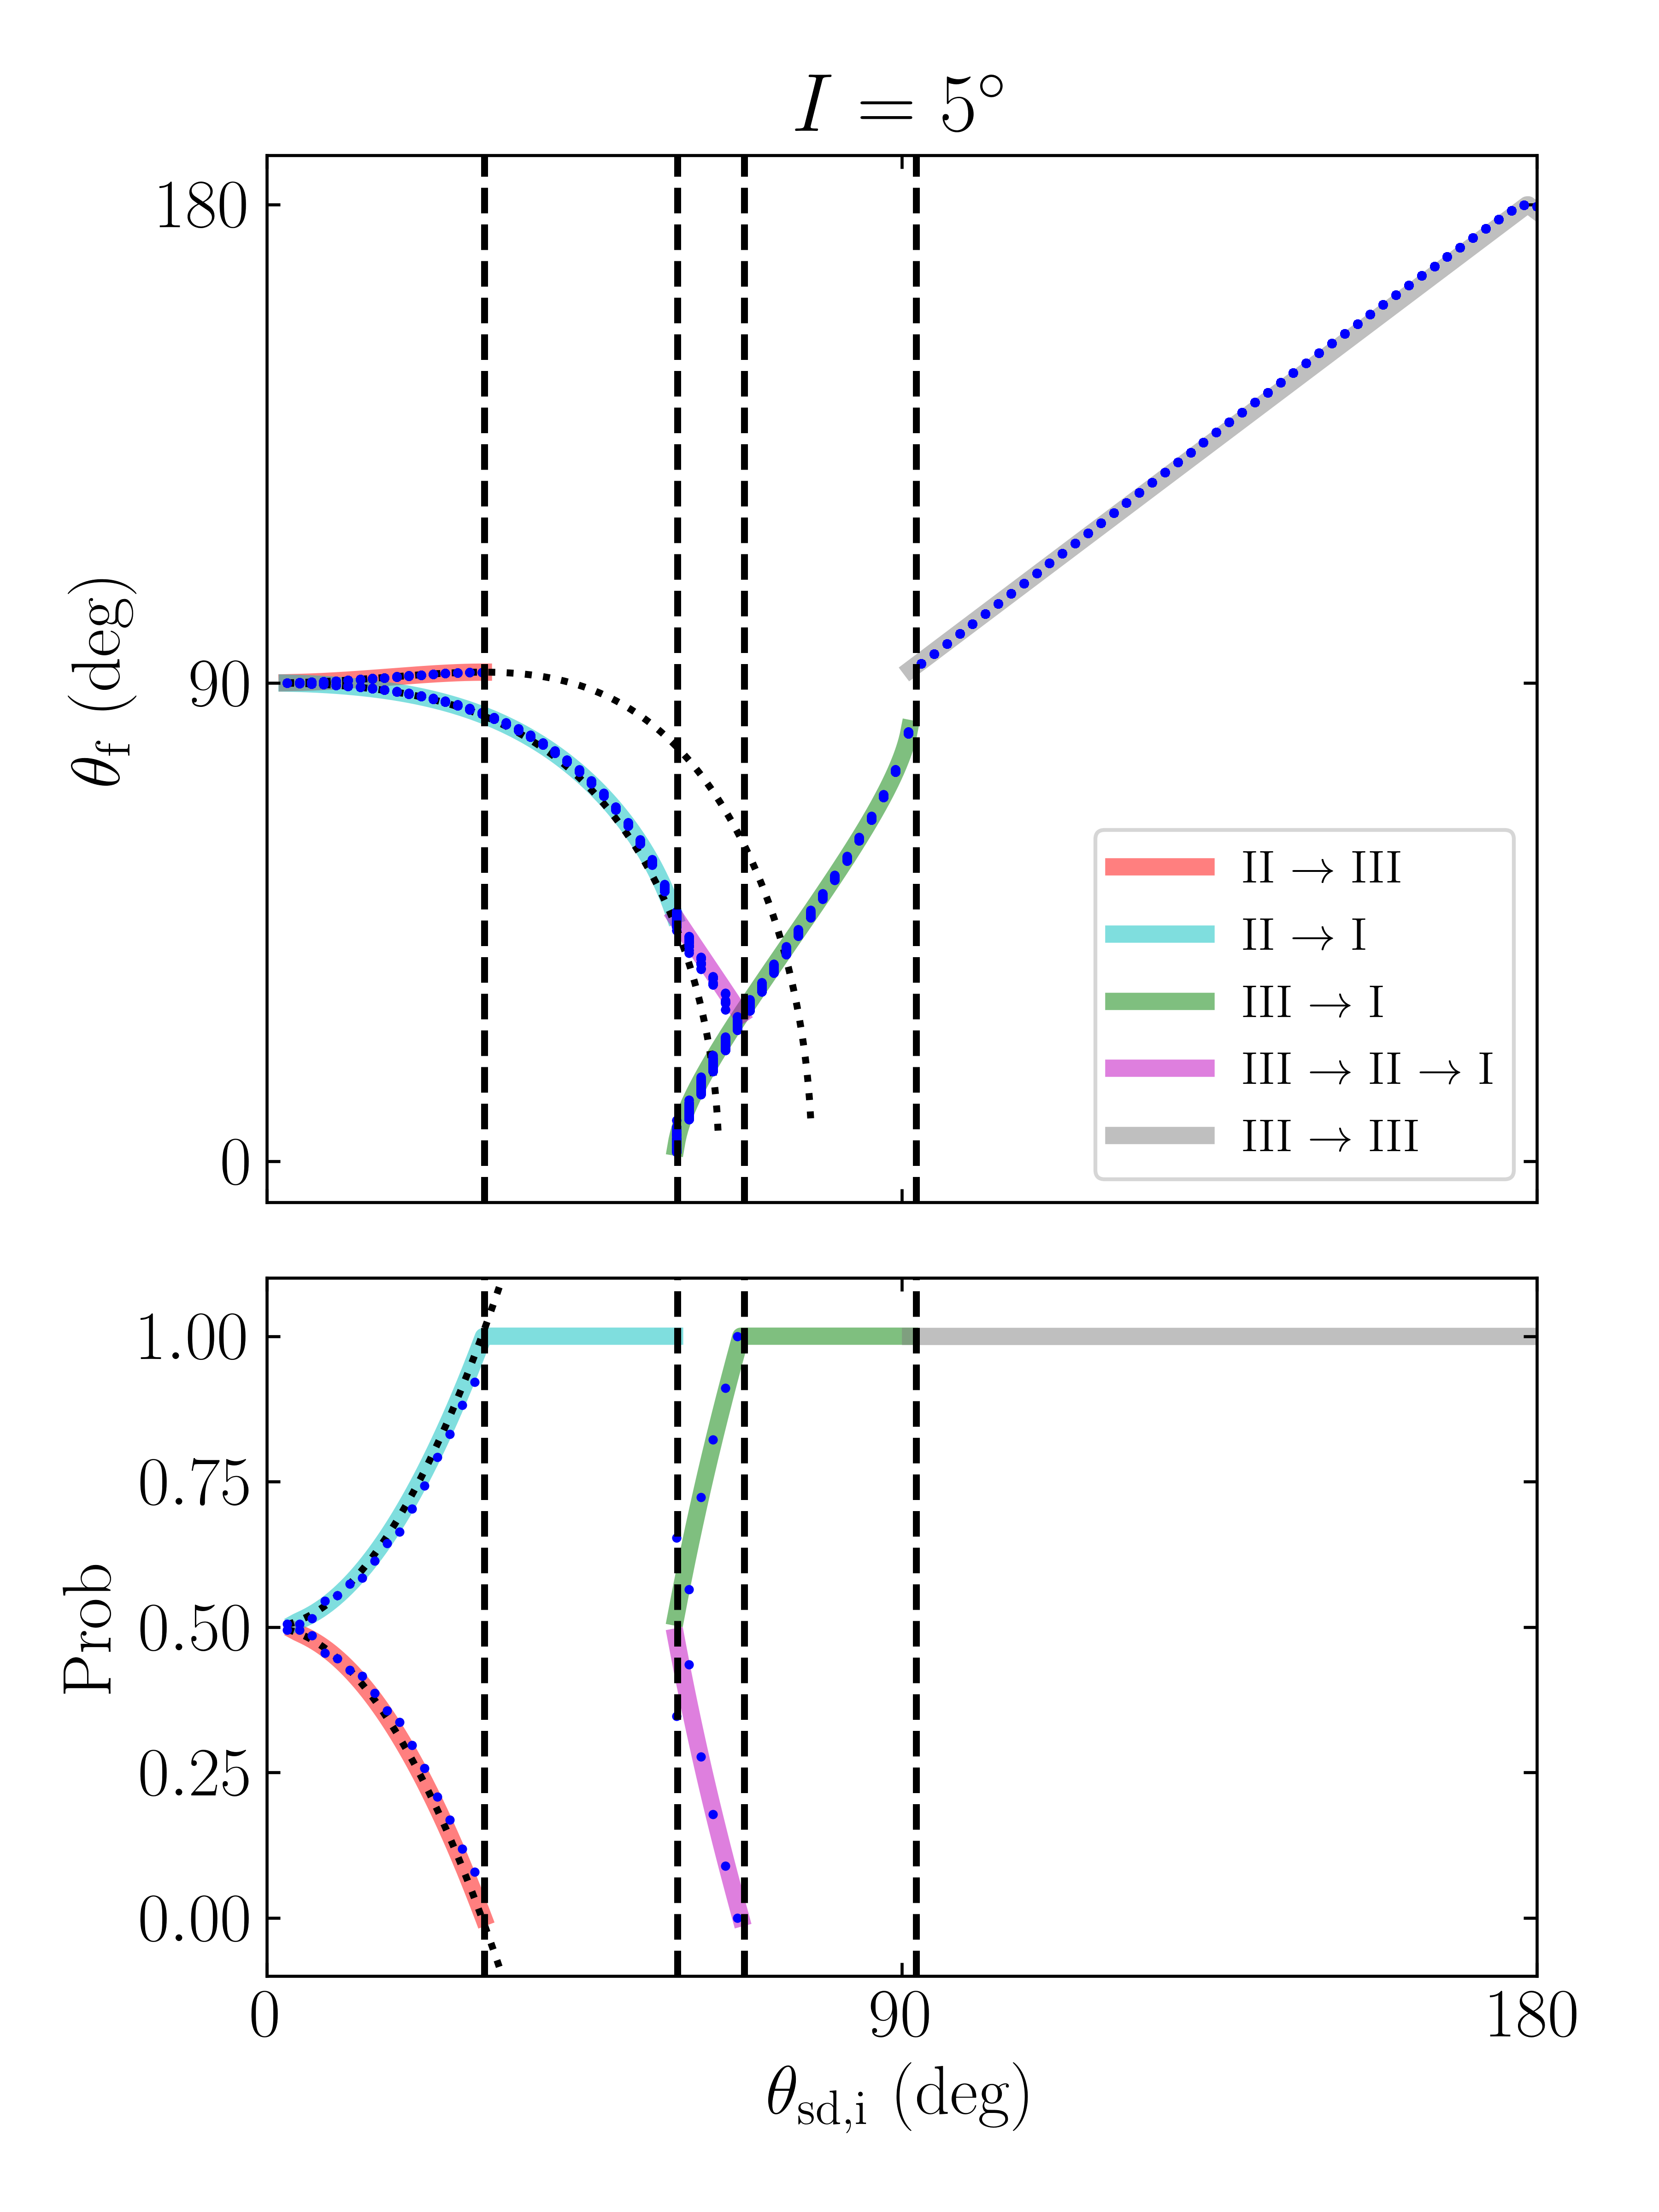
\includegraphics[width=0.7\textwidth]{../../initial/2_toy2/3_ensemble_05_35.png}
        \caption{$\cos \theta_{sl, f} \approx \pm \frac{\sin^2\theta_{sd,
        i}}{4}$}
    \end{figure}
\end{frame}

\begin{frame}
    \frametitle{Results}
    \framesubtitle{Non-Adiabatic}

    \begin{figure}[t]
        \centering
        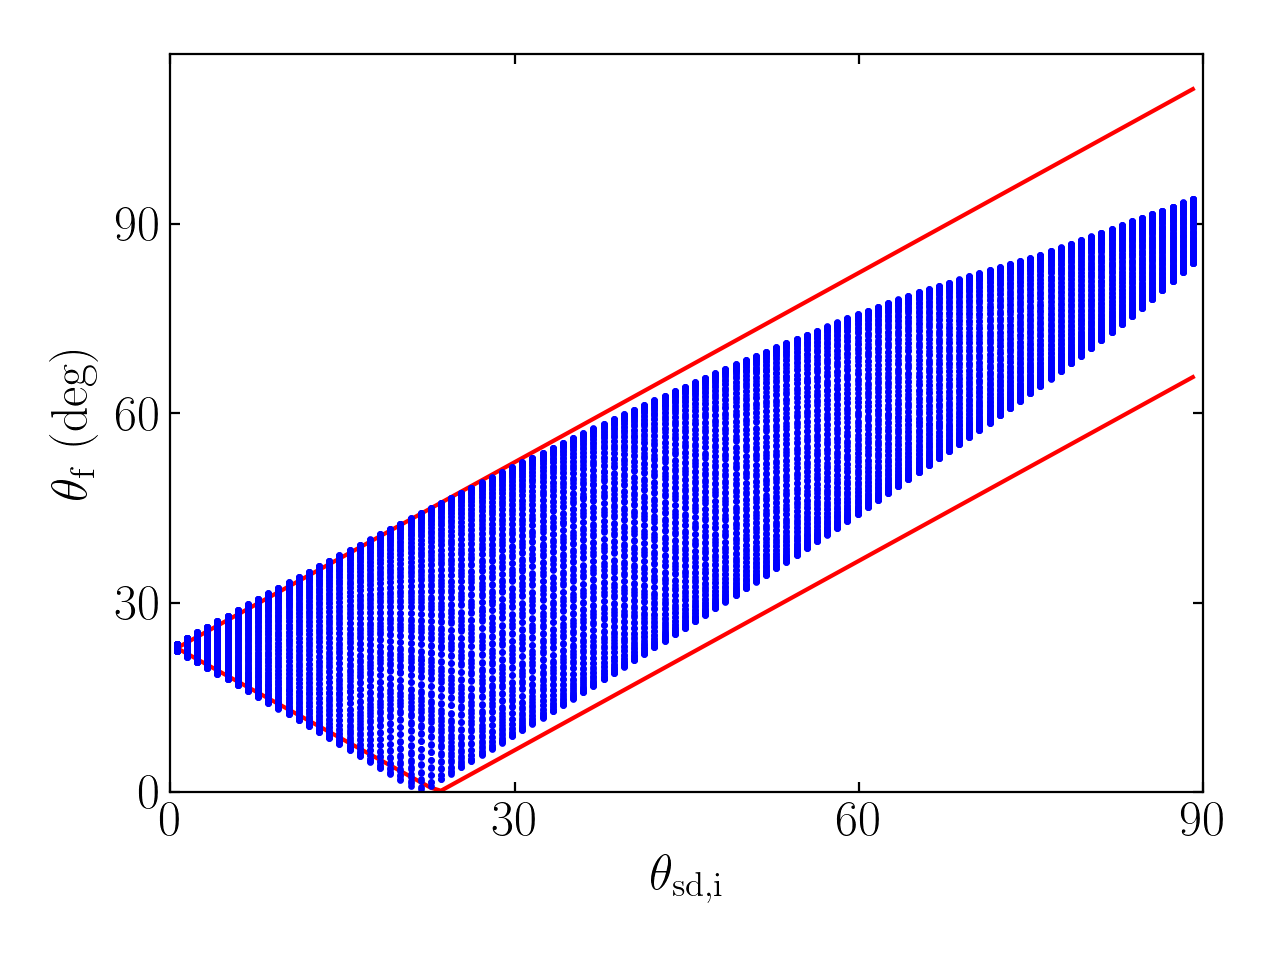
\includegraphics[width=0.7\textwidth]{../../initial/2_toy2/3_ensemble_05_05.png}
        \caption{$\theta_{sl, f} \approx
        \sqrt{2\pi/\alpha\epsilon}\tan I \pm \theta_{sd, i}$.}
    \end{figure}
\end{frame}

\begin{frame}
    \frametitle{Results}
    \framesubtitle{Transition between Adiabaticity/Non-Adiabaticity}

    \begin{figure}[t]
        \centering
        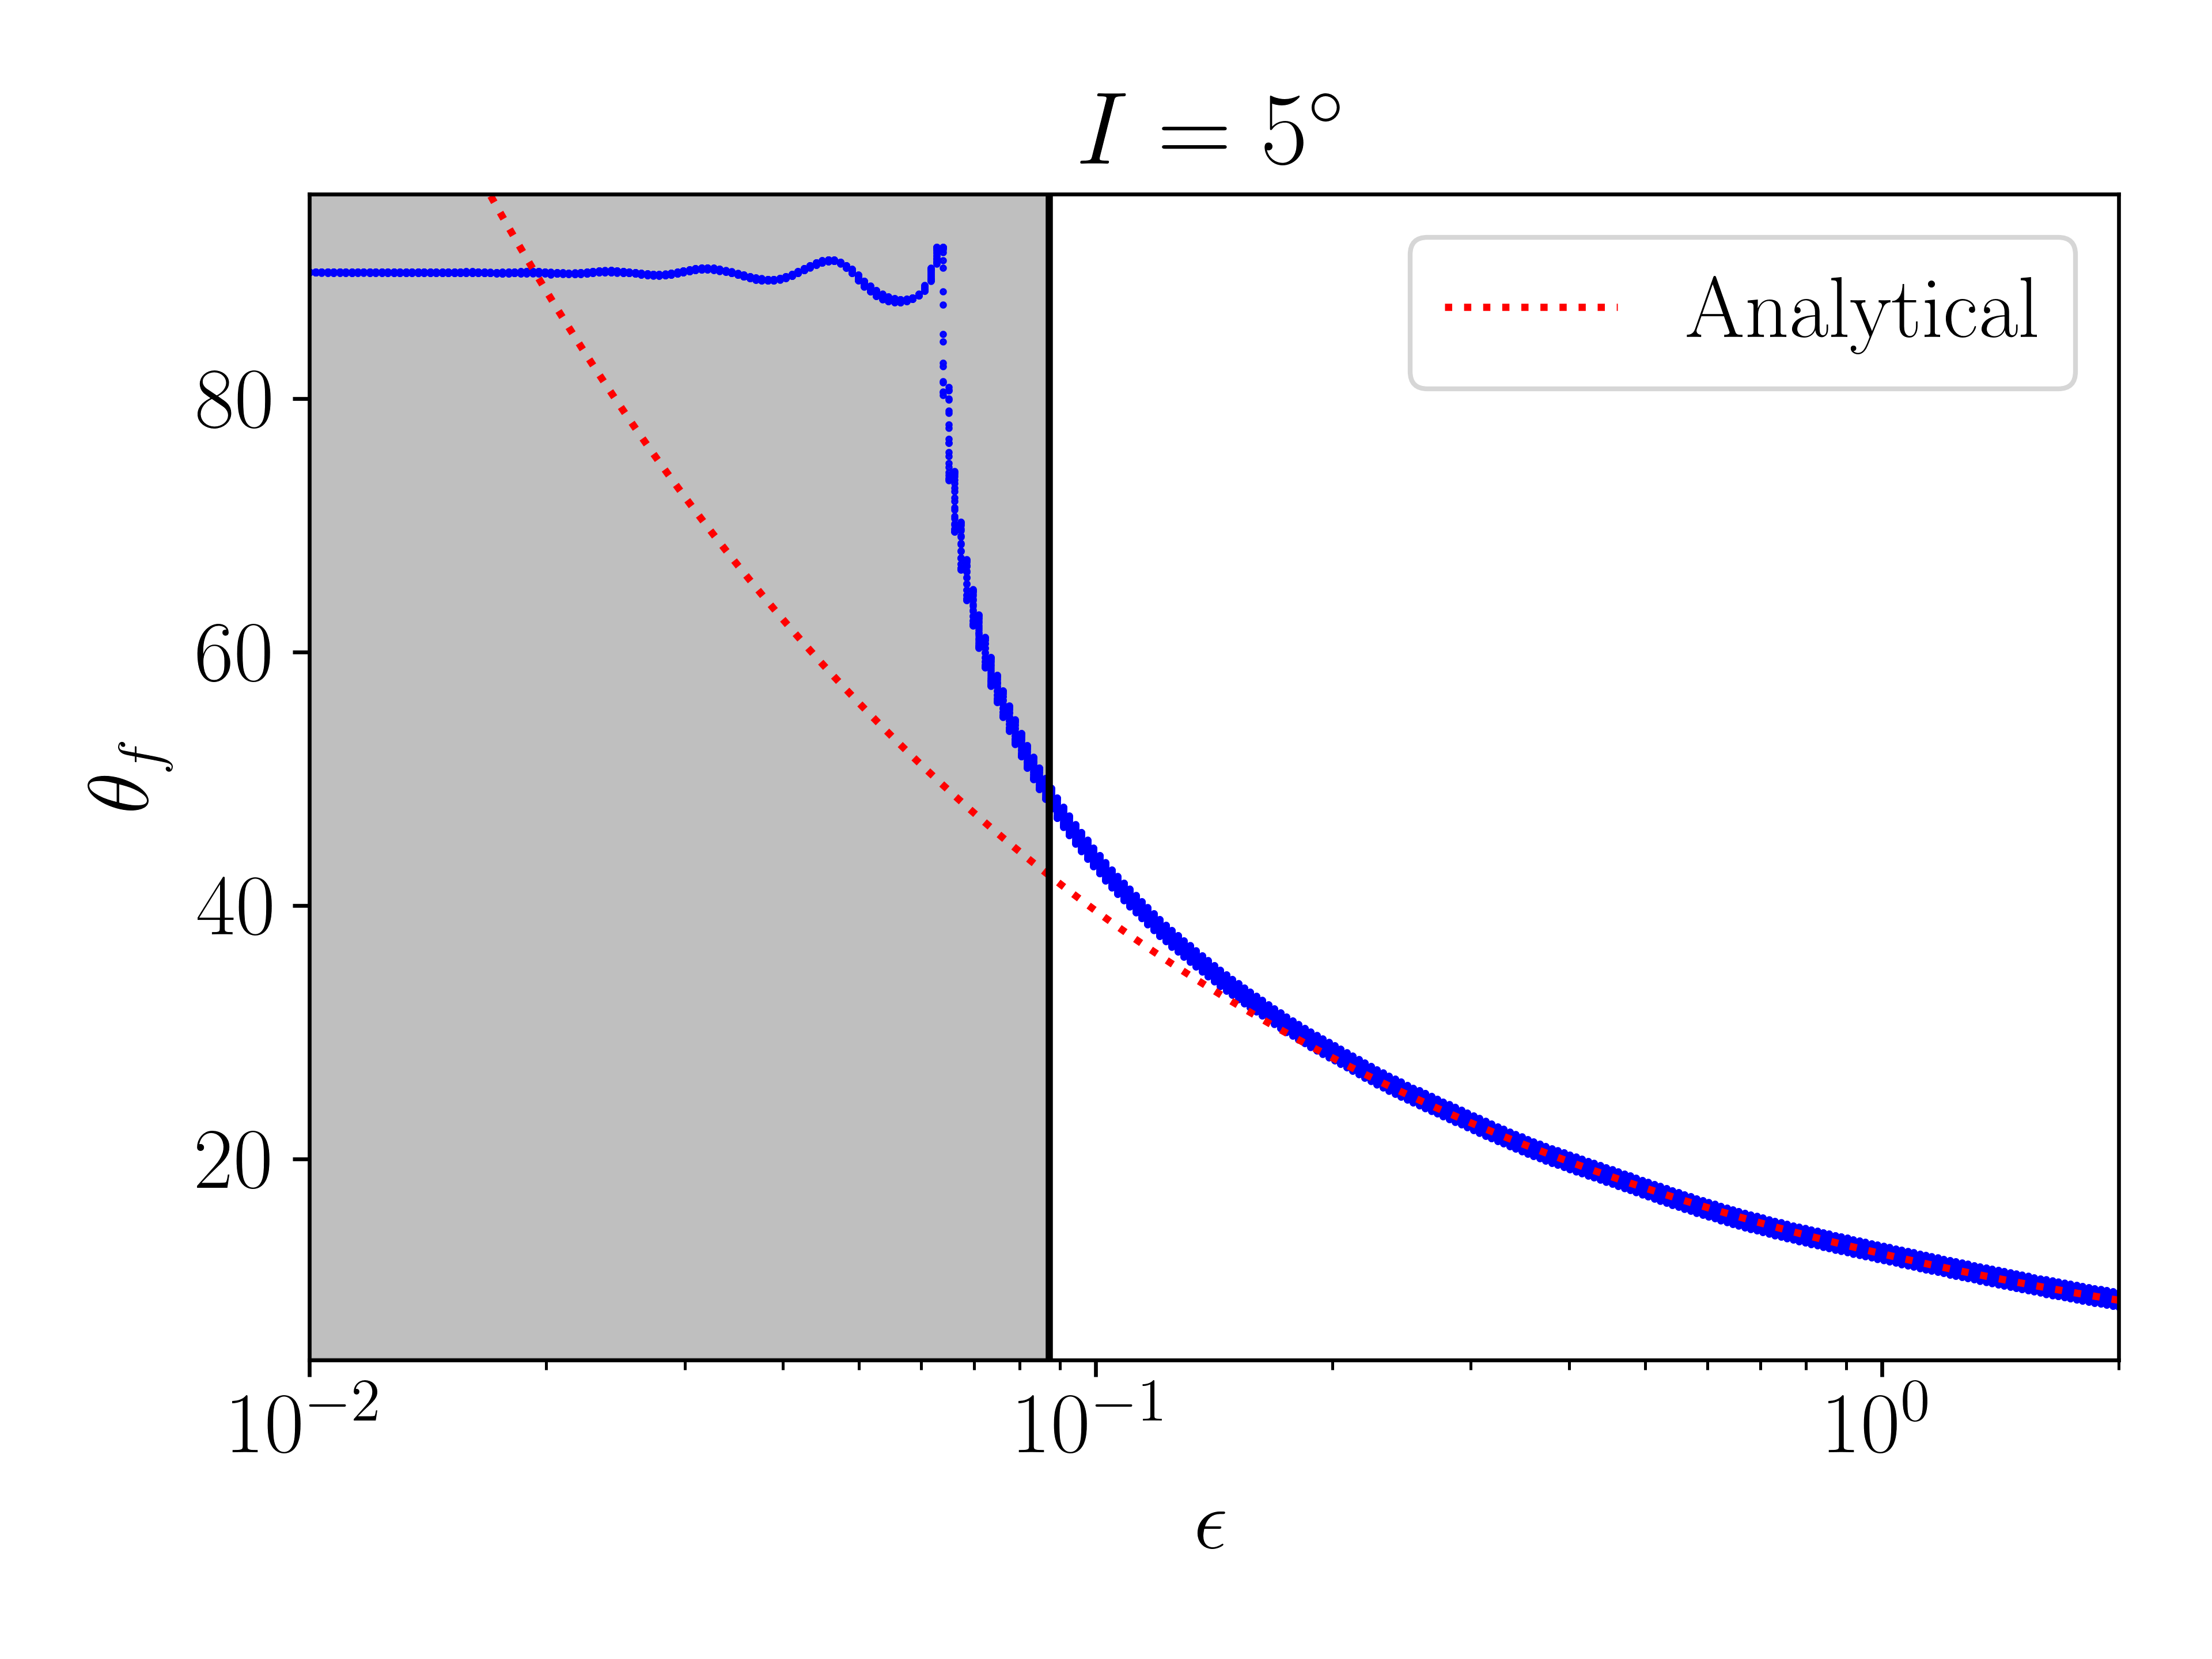
\includegraphics[width=0.7\textwidth]{../../initial/2_toy2/3scan.png}
    \end{figure}
\end{frame}

\end{document}

